% 第9章第3节：对称矩阵特征子空间的扰动（子空间的距离，谱隙控制的偏转界，重特征值与子空间内部的基）。

\section{对称矩阵特征子空间的扰动}
\label{sec:ls-subspace-sensitivity}

即使特征值的绝对误差很小，按这些特征值选出的方向也可能变化很大。本节研究：在给定的误差预算下，原来选出的特征子空间能偏转多少。先建立一种不依赖基的选择的子空间距离，再检查目标特征值组与其余特征值之间的间隔。

\subsection{子空间的距离}

比较特征向量时，比较对象应是子空间本身。特征向量可以变号；特征值重复时，特征空间内部还可以任意换标准正交基，这些都不改变子空间，所以单个基向量的变化不能当作子空间的误差。图~\ref{fig:ls-principal-angles-subspaces}从两条过原点的直线看起：两直线的夹角与方向向量的选取无关；把一条直线的单位方向向量投影到另一条上，投影不掉的部分长度为$\sin\theta$。

\begin{figure}[htbp]
 \centering
 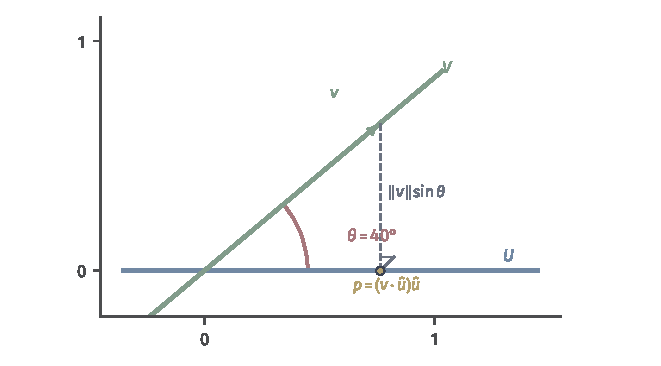
\includegraphics[width=112mm]{figures/00-shared/mathematical-preliminaries-upper/02-linear-spaces/matplotlib/ls-principal-angles-subspaces/ls-principal-angles-subspaces.pdf}
 \caption{两条直线子空间的主夹角。蓝线为$\bm U$、绿线为$\bm V$，红弧为主夹角
 $\theta=40^\circ$；黄点$\bm p$是$\bm v$在$\bm U$上的正交投影，灰虚线为投影
 垂线。$\cos40^\circ\approx0.766$、$\sin40^\circ\approx0.643$，残差长度
 $\lVert\bm v\rVert\sin\theta$即投影不掉的分量。}
 \label{fig:ls-principal-angles-subspaces}
\end{figure}

对一维子空间，若$\bm q,\widetilde{\bm q}$是单位方向向量，则$|\bm q^\top\widetilde{\bm q}|=\cos\theta$。高维子空间之间有多个夹角，由交叉内积矩阵的奇异值给出。
\begin{definition}[主夹角]
\label{def:matrix-analysis-principal-angles}
设$\bm Q,\widetilde{\bm Q}\in\mathbb R^{d\times r}$列标准正交，分别张成$r$维子空间。交叉矩阵$\bm Q^\top\widetilde{\bm Q}$的奇异值记为$\cos\theta_1\geq\dots\geq\cos\theta_r$，$0\leq\theta_1\leq\cdots\leq\theta_r\leq\pi/2$，这些$\theta_i$称为两个子空间的\term{主夹角}（principal angles）。
\end{definition}
这些奇异值都在$[0,1]$内，因为$\lVert\bm Q^\top\widetilde{\bm Q}\rVert_2\leq\lVert\bm Q\rVert_2\lVert\widetilde{\bm Q}\rVert_2=1$，所以$\theta_i$有定义。换基相当于把$\bm Q$、$\widetilde{\bm Q}$分别右乘$r$阶正交矩阵$\bm R$、$\widetilde{\bm R}$，交叉矩阵变为$\bm R^\top(\bm Q^\top\widetilde{\bm Q})\widetilde{\bm R}$，奇异值不变，所以主夹角只依赖两个子空间。最大主夹角$\theta_r$记为$\theta_{\max}$。

主夹角的正弦度量一个子空间伸出另一个子空间的部分，它们也可以直接读出，并与正交投影之差联系起来。设$\widetilde{\bm Q}_\perp\in\mathbb R^{d\times(d-r)}$的列是$\widetilde{\bm Q}$列空间正交补的标准正交基，记
\[
 \bm C=\widetilde{\bm Q}^\top\bm Q,\qquad\bm X=\widetilde{\bm Q}_\perp^\top\bm Q ,
\]
再记两个子空间上的正交投影为$\bm P=\bm Q\bm Q^\top$、$\widetilde{\bm P}=\widetilde{\bm Q}\widetilde{\bm Q}^\top$，它们与基的选取无关。
\begin{theorem}[主夹角的正弦与投影之差]
\label{thm:ls-principal-angle-projection}
在上述记号下，$\bm X^\top\bm X=\bm I-\bm C^\top\bm C$，其特征值为$\sin^2\theta_1,\ldots,\sin^2\theta_r$，并且
\[
 \tfrac12\lVert\bm P-\widetilde{\bm P}\rVert_{\mathrm F}^2=\sum_{i=1}^r\sin^2\theta_i=\lVert\bm X\rVert_{\mathrm F}^2 .
\]
\end{theorem}
\begin{proof}
$[\widetilde{\bm Q},\widetilde{\bm Q}_\perp]$是正交矩阵，所以对任意$\bm a\in\mathbb R^r$，把$\bm Q\bm a$分解到$\widetilde{\bm Q}$的列空间与其正交补，由勾股定理，
\[
 \lVert\bm C\bm a\rVert_2^2+\lVert\bm X\bm a\rVert_2^2=\lVert\bm Q\bm a\rVert_2^2=\lVert\bm a\rVert_2^2 .
\]
即对称矩阵$\bm X^\top\bm X$与$\bm I-\bm C^\top\bm C$的二次型处处相等。对称矩阵由其二次型唯一确定（用$\bm a+\bm b$与$\bm a-\bm b$的二次型之差可以读出$\bm a^\top\bm M\bm b$），所以$\bm X^\top\bm X=\bm I-\bm C^\top\bm C$。$\bm C$是交叉矩阵$\bm Q^\top\widetilde{\bm Q}$的转置，$\bm C^\top\bm C$的特征值是$\cos^2\theta_i$，所以$\bm X^\top\bm X$的特征值是$1-\cos^2\theta_i=\sin^2\theta_i$，且$\lVert\bm X\rVert_{\mathrm F}^2=\operatorname{tr}(\bm X^\top\bm X)=\sum_i\sin^2\theta_i$。

再算投影之差。$\bm P$、$\widetilde{\bm P}$对称且$\bm P^2=\bm P$、$\widetilde{\bm P}^2=\widetilde{\bm P}$，$\operatorname{tr}\bm P=\operatorname{tr}(\bm Q^\top\bm Q)=r$，同样$\operatorname{tr}\widetilde{\bm P}=r$。于是
\[
 \begin{aligned}
 \lVert\bm P-\widetilde{\bm P}\rVert_{\mathrm F}^2
 &=\operatorname{tr}\bigl((\bm P-\widetilde{\bm P})^2\bigr)\\
 &=\operatorname{tr}\bm P-2\operatorname{tr}(\bm P\widetilde{\bm P})+\operatorname{tr}\widetilde{\bm P}\\
 &=2r-2\operatorname{tr}(\bm P\widetilde{\bm P}).
 \end{aligned}
\]
由迹的循环性，$\operatorname{tr}(\bm P\widetilde{\bm P})=\operatorname{tr}(\widetilde{\bm Q}^\top\bm Q\bm Q^\top\widetilde{\bm Q})=\lVert\bm Q^\top\widetilde{\bm Q}\rVert_{\mathrm F}^2=\sum_i\cos^2\theta_i$，代入得$\lVert\bm P-\widetilde{\bm P}\rVert_{\mathrm F}^2=2\sum_i(1-\cos^2\theta_i)=2\sum_i\sin^2\theta_i$。
\end{proof}
Frobenius范数汇总了所有主夹角，反映整体偏转。只关心最坏的那个方向时，用谱范数，它恰好读出最大主夹角。
\begin{theorem}[投影之差的谱范数]
\label{thm:ls-projection-spectral-distance}
在定理~\ref{thm:ls-principal-angle-projection}的记号下，
\[
 \lVert\bm P-\widetilde{\bm P}\rVert_2=\lVert\bm X\rVert_2=\sin\theta_{\max}.
\]
\end{theorem}
\begin{proof}
由定理~\ref{thm:ls-principal-angle-projection}，$\bm X^\top\bm X$的最大特征值是$\sin^2\theta_{\max}$，所以$\lVert\bm X\rVert_2=\sin\theta_{\max}$。

再设$\bm Q_\perp\in\mathbb R^{d\times(d-r)}$的列是$\bm Q$列空间正交补的标准正交基，于是$\bm I-\bm P=\bm Q_\perp\bm Q_\perp^\top$、$\bm I-\widetilde{\bm P}=\widetilde{\bm Q}_\perp\widetilde{\bm Q}_\perp^\top$。先说明两个算子范数。列标准正交的矩阵保持长度，行标准正交的矩阵不增加长度，并在其行空间上保持长度，所以
\[
 \lVert(\bm I-\widetilde{\bm P})\bm P\rVert_2
 =\lVert\widetilde{\bm Q}_\perp(\widetilde{\bm Q}_\perp^\top\bm Q)\bm Q^\top\rVert_2
 =\lVert\bm X\rVert_2 .
\]
同理$\lVert(\bm I-\bm P)\widetilde{\bm P}\rVert_2=\lVert\bm Q_\perp^\top\widetilde{\bm Q}\rVert_2$。把定理~\ref{thm:ls-principal-angle-projection}中两个子空间的角色交换，交叉矩阵变为$\widetilde{\bm Q}^\top\bm Q$，它与原交叉矩阵互为转置，奇异值相同，所以$\bm Q_\perp^\top\widetilde{\bm Q}$的最大奇异值同样是$\sin\theta_{\max}$。

上界：直接展开可验证
\[
 \bm P-\widetilde{\bm P}=\bm P(\bm I-\widetilde{\bm P})-(\bm I-\bm P)\widetilde{\bm P}.
\]
对任意$\bm z$，右端第一项落在$\bm Q$的列空间中，第二项落在其正交补中，由勾股定理，
\[
 \begin{aligned}
 \lVert(\bm P-\widetilde{\bm P})\bm z\rVert_2^2
 &=\lVert\bm P(\bm I-\widetilde{\bm P})\bm z\rVert_2^2+\lVert(\bm I-\bm P)\widetilde{\bm P}\bm z\rVert_2^2\\
 &\leq\sin^2\theta_{\max}\bigl(\lVert(\bm I-\widetilde{\bm P})\bm z\rVert_2^2+\lVert\widetilde{\bm P}\bm z\rVert_2^2\bigr)\\
 &=\sin^2\theta_{\max}\lVert\bm z\rVert_2^2 .
 \end{aligned}
\]
这里第二行用到$\bm P(\bm I-\widetilde{\bm P})=\bigl((\bm I-\widetilde{\bm P})\bm P\bigr)^\top$，转置不改变谱范数，并对两项分别使用上面的范数等式；第三行再用勾股定理。

下界：取单位向量$\bm a\in\mathbb R^r$使$\lVert\bm X\bm a\rVert_2=\lVert\bm X\rVert_2$（取$\bm X$的第一右奇异向量），令$\bm z=\bm Q\bm a$，则$\lVert\bm z\rVert_2=1$，$\bm P\bm z=\bm z$，
\[
 (\bm P-\widetilde{\bm P})\bm z=(\bm I-\widetilde{\bm P})\bm Q\bm a=\widetilde{\bm Q}_\perp\bm X\bm a ,
\]
长度为$\lVert\bm X\bm a\rVert_2=\sin\theta_{\max}$。两方面合起来即得结论。
\end{proof}

\subsection{谱隙控制的偏转界}

现在比较特征子空间。设$\bm S$、$\widetilde{\bm S}=\bm S+\bm E\in\mathbb R^{d\times d}$实对称，取$1\leq k<d$，比较两者前$k$个特征值对应的子空间。要使比较有意义，原矩阵的目标特征值组必须与其余特征值分开：设截断处的\term{谱隙}（spectral gap）
\[
 \delta=\lambda_k(\bm S)-\lambda_{k+1}(\bm S)>0 ,
\]
这时$\bm S$前$k$个特征值对应的特征子空间是唯一确定的$k$维子空间。若误差预算满足$\lVert\bm E\rVert_2\leq\varepsilon<\delta/2$，由Weyl界，
\[
 \lambda_k(\widetilde{\bm S})\geq\lambda_k(\bm S)-\varepsilon>\lambda_{k+1}(\bm S)+\varepsilon\geq\lambda_{k+1}(\widetilde{\bm S}),
\]
扰动后截断处仍然严格分开，$\widetilde{\bm S}$前$k$个特征值的特征子空间也唯一确定，两者都是$k$维，可以用主夹角比较。

下面的论证用到的是交叉谱间隔
\[
 \gamma=\lambda_k(\bm S)-\lambda_{k+1}(\widetilde{\bm S}),
\]
即原目标组的最小特征值与扰动后其余特征值的最大者之差。由Weyl界$\lambda_{k+1}(\widetilde{\bm S})\leq\lambda_{k+1}(\bm S)+\varepsilon$，得$\gamma\geq\delta-\varepsilon>0$。

记$\bm Q\in\mathbb R^{d\times k}$的列是$\bm S$前$k$个特征值的标准正交特征向量，$\bm\Lambda_1=\operatorname{diag}(\lambda_1(\bm S),\ldots,\lambda_k(\bm S))$；$\widetilde{\bm Q}$的列是$\widetilde{\bm S}$前$k$个特征值的标准正交特征向量，$\widetilde{\bm Q}_\perp$的列是其余的标准正交特征向量，对应特征值组成对角矩阵$\widetilde{\bm\Lambda}_2=\operatorname{diag}(\lambda_{k+1}(\widetilde{\bm S}),\ldots,\lambda_d(\widetilde{\bm S}))$。令$\bm X=\widetilde{\bm Q}_\perp^\top\bm Q$，由定理~\ref{thm:ls-principal-angle-projection}，它的Frobenius范数平方就是两个子空间主夹角正弦的平方和。

\begin{theorem}[特征子空间偏转的Frobenius界]
\label{thm:ls-gap-subspace-frobenius}
在上述记号下，若$\gamma=\lambda_k(\bm S)-\lambda_{k+1}(\widetilde{\bm S})>0$，则$\bm Q$与$\widetilde{\bm Q}$张成的子空间的主夹角$\theta_1,\ldots,\theta_k$满足
\[
 \begin{aligned}
 \Bigl(\sum_{i=1}^k\sin^2\theta_i\Bigr)^{1/2}
 &=\lVert\bm X\rVert_{\mathrm F}\\
 &\leq\frac{\lVert\widetilde{\bm Q}_\perp^\top\bm E\bm Q\rVert_{\mathrm F}}{\gamma}
 \leq\frac{\lVert\bm E\bm Q\rVert_{\mathrm F}}{\gamma}.
 \end{aligned}
\]
\end{theorem}
\begin{proof}
由特征关系$\widetilde{\bm Q}_\perp^\top\widetilde{\bm S}=\widetilde{\bm\Lambda}_2\widetilde{\bm Q}_\perp^\top$（对$\widetilde{\bm S}\widetilde{\bm Q}_\perp=\widetilde{\bm Q}_\perp\widetilde{\bm\Lambda}_2$取转置）右乘$\bm Q$，又由$\bm S\bm Q=\bm Q\bm\Lambda_1$左乘$\widetilde{\bm Q}_\perp^\top$，两式相减，并用$\widetilde{\bm S}-\bm S=\bm E$，得
\[
 \widetilde{\bm\Lambda}_2\bm X-\bm X\bm\Lambda_1=\widetilde{\bm Q}_\perp^\top\bm E\bm Q .
\]
这是关于$\bm X$的线性方程，两侧的系数矩阵都是对角的，可以逐元素读出。把$\bm X$的行用$j=k+1,\ldots,d$编号、列用$i=1,\ldots,k$编号，第$(j,i)$元满足
\[
 \bigl(\lambda_j(\widetilde{\bm S})-\lambda_i(\bm S)\bigr)X_{j,i}=(\widetilde{\bm Q}_\perp^\top\bm E\bm Q)_{j,i}.
\]
由降序，$i\leq k<j$时$\lambda_i(\bm S)-\lambda_j(\widetilde{\bm S})\geq\lambda_k(\bm S)-\lambda_{k+1}(\widetilde{\bm S})=\gamma>0$，所以$|X_{j,i}|\leq|(\widetilde{\bm Q}_\perp^\top\bm E\bm Q)_{j,i}|/\gamma$。逐元素平方求和，得第一个不等式。$\widetilde{\bm Q}_\perp^\top$的行标准正交，对任意向量$\bm m$有$\lVert\widetilde{\bm Q}_\perp^\top\bm m\rVert_2\leq\lVert\bm m\rVert_2$，按列应用于$\bm E\bm Q$即得第二个不等式。等式部分来自定理~\ref{thm:ls-principal-angle-projection}。
\end{proof}
证明中出现的方程同时含有左乘和右乘未知矩阵的两项，这类方程称为Sylvester方程，第~\ref{sec:ls-matrix-equations}节专门研究它；这里两侧系数都是对角矩阵，逐元素相除就够了。由$\lVert\bm E\bm Q\rVert_{\mathrm F}\leq\sqrt k\,\lVert\bm E\rVert_2$，右端不超过$\sqrt k\,\lVert\bm E\rVert_2/\gamma$。

对谱范数，即最大主夹角，也有同型的结论。它不是上面Frobenius估计的直接推论：由Frobenius界只能得到带因子$\sqrt k$的估计。去掉这个因子要换一种读法：不逐元素相除，而是用$\bm X$的最大奇异方向从两侧检验同一个矩阵方程。
\begin{theorem}[Davis--Kahan谱隙界]
\label{thm:ls-davis-kahan}
在定理~\ref{thm:ls-gap-subspace-frobenius}的条件下，
\begin{equation}
 \lVert\widetilde{\bm P}-\bm P\rVert_2=\sin\theta_{\max}
 \leq\frac{\lVert\bm E\bm Q\rVert_2}{\gamma}\leq\frac{\lVert\bm E\rVert_2}{\gamma}.
 \label{eq:matrix-analysis-eigenvector-gap-bound}
\end{equation}
\end{theorem}
\begin{proof}
由定理~\ref{thm:ls-projection-spectral-distance}，$\lVert\widetilde{\bm P}-\bm P\rVert_2=\sin\theta_{\max}=\lVert\bm X\rVert_2$，记$s=\lVert\bm X\rVert_2$。$s=0$时结论成立，下设$s>0$。取$\bm X$的第一右、左奇异向量$\bm a\in\mathbb R^k$、$\bm b\in\mathbb R^{d-k}$，它们是单位向量，满足$\bm X\bm a=s\bm b$、$\bm X^\top\bm b=s\bm a$。用$\bm b^\top$左乘、$\bm a$右乘定理~\ref{thm:ls-gap-subspace-frobenius}证明中的方程$\widetilde{\bm\Lambda}_2\bm X-\bm X\bm\Lambda_1=\widetilde{\bm Q}_\perp^\top\bm E\bm Q$，左端为
\[
 \begin{aligned}
 &\bm b^\top\widetilde{\bm\Lambda}_2(\bm X\bm a)-(\bm X^\top\bm b)^\top\bm\Lambda_1\bm a\\
 &\quad=s\bigl(\bm b^\top\widetilde{\bm\Lambda}_2\bm b-\bm a^\top\bm\Lambda_1\bm a\bigr).
 \end{aligned}
\]
$\bm\Lambda_1$的对角元都不小于$\lambda_k(\bm S)$，$\bm a$是单位向量，所以
\[
 \bm a^\top\bm\Lambda_1\bm a=\sum_i\lambda_i(\bm S)a_i^2\geq\lambda_k(\bm S);
\]
同理$\bm b^\top\widetilde{\bm\Lambda}_2\bm b\leq\lambda_{k+1}(\widetilde{\bm S})$。于是左端的绝对值至少为$s\gamma$。右端的绝对值满足
\[
 |\bm b^\top\widetilde{\bm Q}_\perp^\top\bm E\bm Q\bm a|
 \leq\lVert\widetilde{\bm Q}_\perp\bm b\rVert_2\,\lVert\bm E\bm Q\bm a\rVert_2
 \leq\lVert\bm E\bm Q\rVert_2 ,
\]
其中用到$\lVert\widetilde{\bm Q}_\perp\bm b\rVert_2=\lVert\bm b\rVert_2=1$。所以$s\gamma\leq\lVert\bm E\bm Q\rVert_2$，即第一个不等式。最后$\lVert\bm E\bm Q\bm a\rVert_2\leq\lVert\bm E\rVert_2\lVert\bm Q\bm a\rVert_2=\lVert\bm E\rVert_2$，得第二个不等式。
\end{proof}
这个证明只用到单侧的谱分离：原目标组的特征值都不小于$\lambda_k(\bm S)$，扰动后其余的特征值都不大于$\lambda_{k+1}(\widetilde{\bm S})$。这正是本节使用的情形；目标组位于谱的中间、两侧都有其余特征值时，需要另作处理，本节不使用。

把交叉间隔换成事先就能检查的量：若已知原谱隙$\delta$且$\lVert\bm E\rVert_2\leq\varepsilon<\delta/2$，前面已得$\gamma\geq\delta-\varepsilon$，于是
\begin{equation}
 \lVert\widetilde{\bm P}-\bm P\rVert_2\leq\frac{\varepsilon}{\delta-\varepsilon}\leq\frac{2\varepsilon}{\delta},
 \label{eq:ls-gap-subspace-budget}
\end{equation}
后一个不等号用到$\delta-\varepsilon>\delta/2$。谱隙在分母上：谱隙越小，同样的扰动能使子空间转过的角度越大。若已经知道交叉间隔$\gamma>0$，也可以直接使用带$\gamma$的形式；原谱隙与误差预算只是一组便于事先检查的充分条件。

下面的二维例子可以精确算出转角，并说明子空间的敏感程度不能由矩阵条件数判断。
\begin{example}[谱隙与特征方向的转角]
\label{ex:ls-gap-direction-rotation}
取$\bm S=\operatorname{diag}(1+\delta,1)$与交叉扰动
\[
 \bm E=t\begin{bmatrix}0&1\\1&0\end{bmatrix},\qquad\delta>0,\ t\geq0 .
\]
$\bm S$的谱隙为$\delta$，最大特征方向是$\bm e_1$，$\lVert\bm E\rVert_2=t$。扰动只在非对角位置把两个坐标耦合起来，我们要算出最大特征方向因此转过多大的角度。为了求扰动后的特征向量，先把矩阵写成单位矩阵的倍数加一个迹为零的部分：
\[
 \bm S+\bm E=\bigl(1+\tfrac\delta2\bigr)\bm I+\bm M,\qquad
 \bm M=\begin{bmatrix}\delta/2&t\\t&-\delta/2\end{bmatrix}.
\]
加上单位矩阵的倍数只平移特征值，不改变特征向量，所以只需研究$\bm M$。记$r=\sqrt{\delta^2/4+t^2}>0$，取$\theta\in[0,\pi/4)$满足$\cos2\theta=\delta/(2r)$、$\sin2\theta=t/r$，即
\[
 \tan2\theta=\frac{2t}{\delta}.
\]
于是$\bm M=r\left[\begin{smallmatrix}\cos2\theta&\sin2\theta\\\sin2\theta&-\cos2\theta\end{smallmatrix}\right]$，由两角差公式，
\[
 \bm M\begin{bmatrix}\cos\theta\\\sin\theta\end{bmatrix}
 =r\begin{bmatrix}\cos(2\theta-\theta)\\\sin(2\theta-\theta)\end{bmatrix}
 =r\begin{bmatrix}\cos\theta\\\sin\theta\end{bmatrix}.
\]
$\bm M$的迹为零，另一个特征值是$-r$。所以$\bm S+\bm E$的特征值为$1+\delta/2\pm r$，最大特征方向从$\bm e_1$转到$(\cos\theta,\sin\theta)^\top$，转角$\theta$满足$\tan2\theta=2t/\delta$。

转角只依赖比值$t/\delta$，与矩阵的条件数无关。$\bm S$的条件数$\kappa_2(\bm S)=1+\delta$，$\delta$小时接近$1$，按第~\ref{sec:ls-perturbation}节的标准是良态的；但取$t=\delta/2$时，$\tan2\theta=1$，$\theta=\pi/8=22.5^\circ$：扰动与谱隙相当，方向就明显偏转。同一扰动下，最大特征值只增加$r-\delta/2\leq t$，符合Weyl界。所以特征值稳定、条件数小，都不能推出特征方向稳定。
\end{example}
与界~\eqref{eq:matrix-analysis-eigenvector-gap-bound}比较：交叉间隔$\gamma=(1+\delta)-(1+\delta/2-r)=\delta/2+r$，界给出$\sin\theta\leq t/(\delta/2+r)$。由$t^2=r^2-\delta^2/4$与$\cos2\theta=\delta/(2r)$可算出
\[
 \sin\theta=\sqrt{\frac{r-\delta/2}{2r}}\leq\sqrt{\frac{r-\delta/2}{r+\delta/2}}=\frac{t}{\delta/2+r},
\]
与界相符；$t\ll\delta$时两端都约为$t/\delta$，界在量级上是准确的。小扰动形式$2\varepsilon/\delta$要求$t<\delta/2$，例中$t=\delta/2$已在这个条件之外，那里只保留精确算例的结论。图~\ref{fig:matrix-analysis-gap-direction}固定$t$，画出最大特征值的增量和转角随谱隙的变化。

\begin{figure}
 \centering
 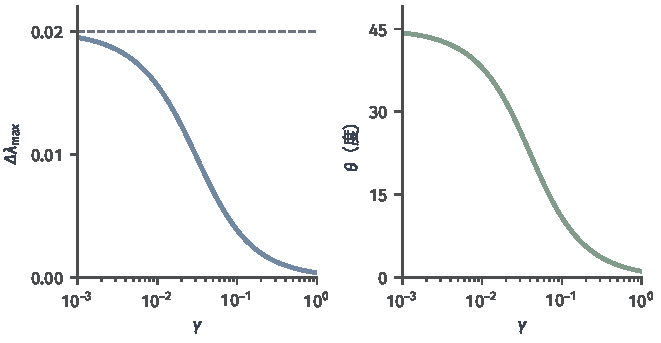
\includegraphics[width=0.92\linewidth]{figures/00-shared/mathematical-preliminaries-upper/02-linear-spaces/matplotlib/matrix-analysis-gap-direction/figure.pdf}
 \caption{谱隙与特征方向的转角（示例~\ref{ex:ls-gap-direction-rotation}，$t=0.02$）。横轴为原谱隙，
 图中记为$\gamma$，即正文的$\delta$。左：最大特征值的增量$r-\delta/2$，始终不超过虚线所示的$t$，
 符合Weyl界；右：最大特征方向的转角$\theta=\tfrac12\arctan(2t/\delta)$。谱隙远大于$t$时转角很小，
 谱隙小于$t$时转角接近$45^\circ$。}
 \label{fig:matrix-analysis-gap-direction}
\end{figure}

\subsection{重特征值与子空间内部的基}

谱隙只需存在于目标特征值组与组外之间，组内的特征值不必彼此分开。取$\bm S=\operatorname{diag}(2,2,0)$与$k=2$，原谱隙$\delta=2-0=2$。由式~\eqref{eq:ls-gap-subspace-budget}，$\lVert\bm E\rVert_2\leq\varepsilon<1$时，前二维特征子空间的最大主夹角满足$\sin\theta_{\max}\leq\varepsilon/(2-\varepsilon)<\varepsilon$，这个平面是稳定的。

但平面内单个特征向量的选择并不稳定：取$\eta>0$，扰动$\eta\bm e_1\bm e_1^\top$使最大特征方向成为$\bm e_1$，扰动$\eta\bm e_2\bm e_2^\top$使它成为$\bm e_2$。无论$\eta$多小，两个结果都相互正交，而前二维子空间始终是$\operatorname{span}\{\bm e_1,\bm e_2\}$。所以不能把子空间内部基的变化解释为整个子空间发生了同样大的变化，反过来，子空间稳定也不保证其中每个基向量稳定。


这两点合起来，对称矩阵所选特征子空间的稳定性只取决于目标组与组外之间的间隙。下一节转向一般方阵，先看特征值本身在缺少对称结构时怎样变化。
